\subsection{16-bit Kogge-Stone Adder}
The Kogge-Stone adder consists of several simple blocks connected in a complex way. The adder has been significantly changed since the high-level design phase. The \textit{yellow} block has been split into two blocks \textit{yellow\_inv\_in} and \textit{yellow\_inv\_out}, which can be seen in Fig. \ref{fig:yellow_opt}. The \textit{yellow\_inv\_in} block takes inverted input signals and gives non-inverting output. The \textit{yellow\_inv\_out} block takes non-inverted intputs and gives inverting output. This arrengement saves a lot of gates. The \textit{yellow\_carry} block has been split in the same way. 

Because of the inverting signals from \textit{yellow\_inv\_out} some \textit{sum} blocks have been replaced with XNOR gates. A couple of inverters have also been added in some places.

All transistors in the adder are minimum sized since the gates have a low fan out.

\begin{figure}[H]
  \centering
  \captionsetup{justification=centering}
  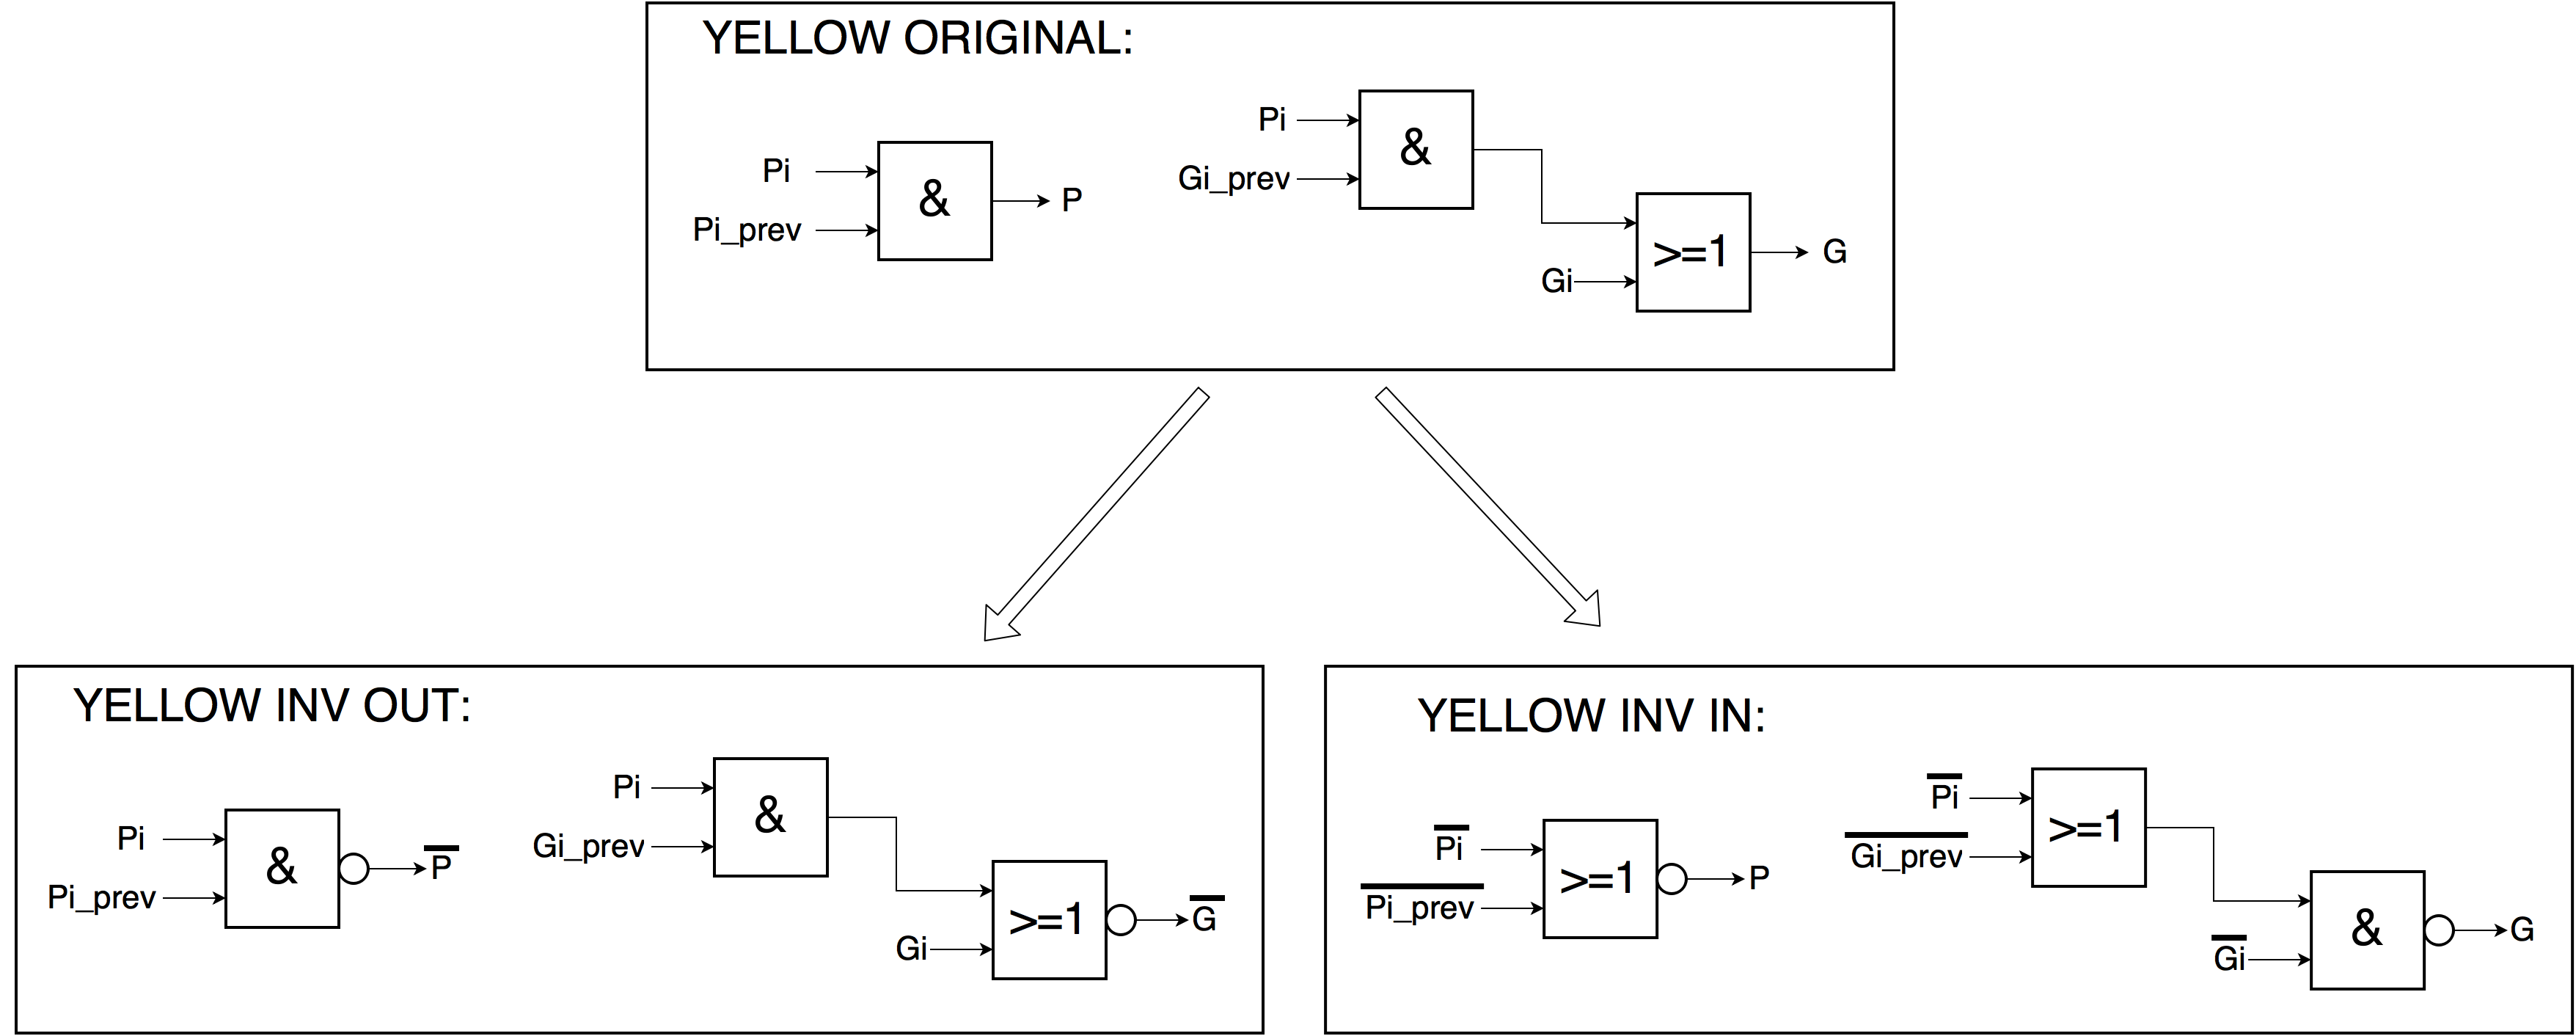
\includegraphics[scale=0.12]{../figures/yellow_opt}
  \caption{The new yellow blocks.} \label{fig:yellow_opt}
\end{figure}

To save space, new switch nets were created for the generate calculation of the \textit{yellow} blocks. The new nets can be seen in Fig. \ref{fig:G_inv_in} and \ref{fig:G_inv_out}. By doing this the transistor count is cut in half. 

\begin{figure}[H]
  \centering
  \captionsetup{justification=centering}
  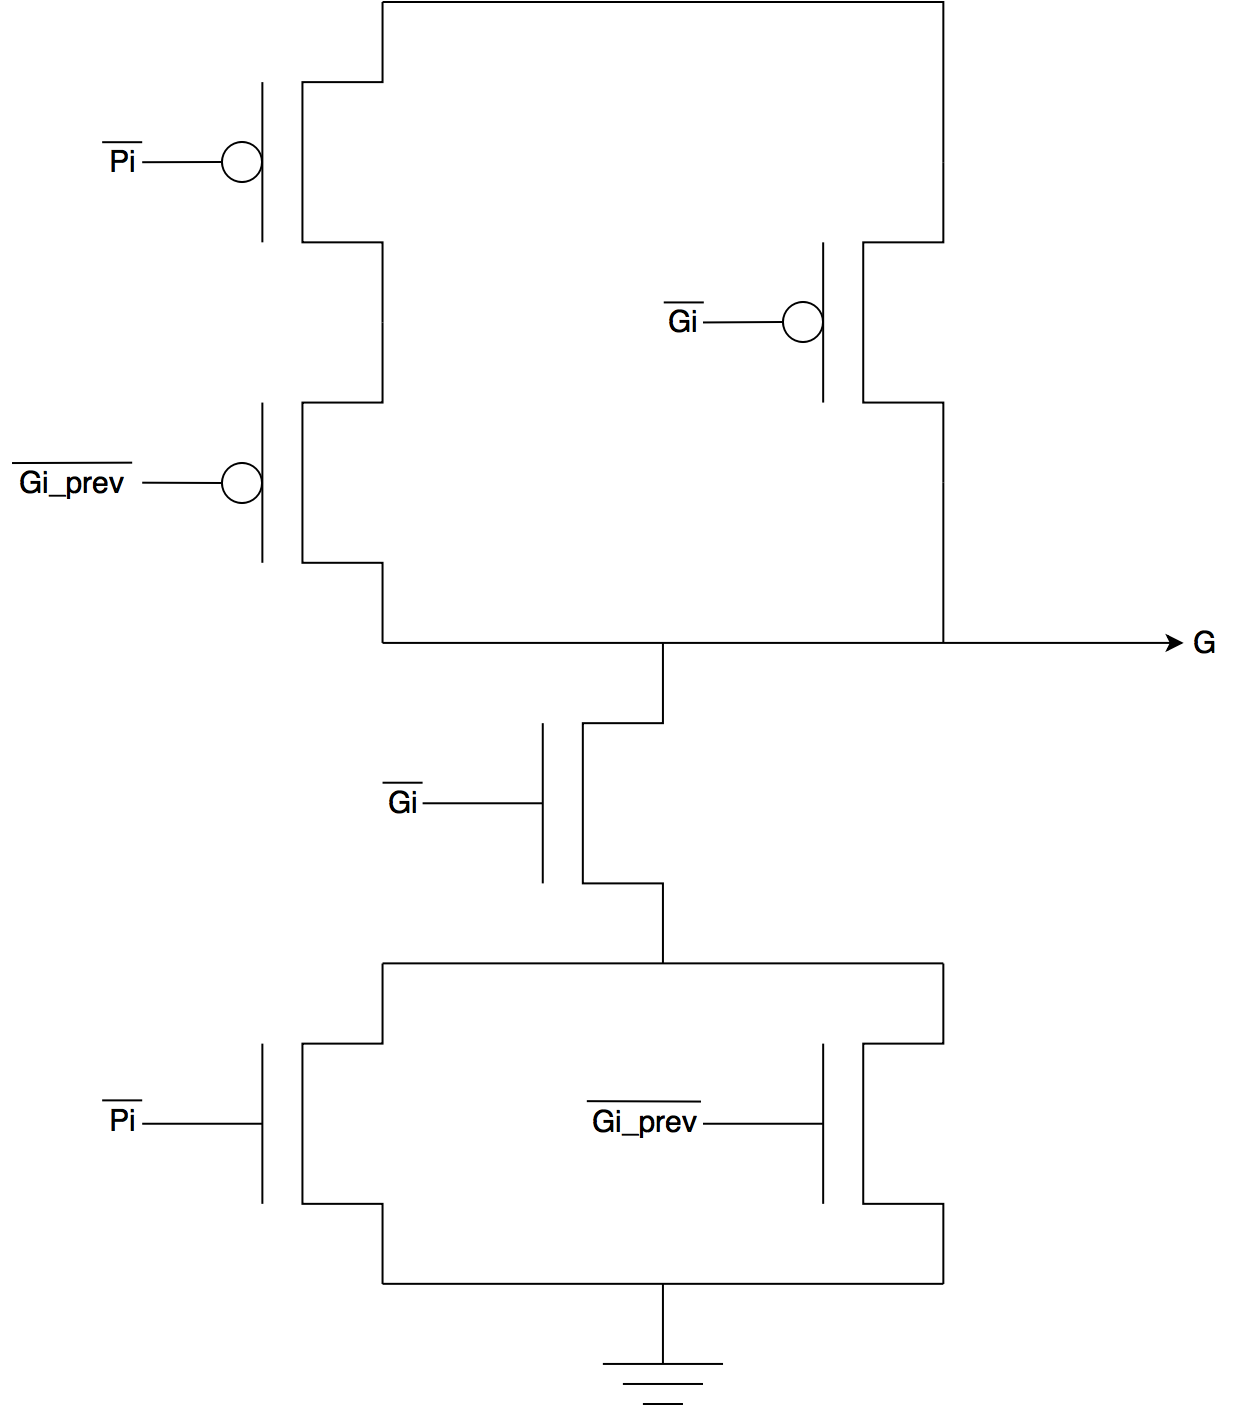
\includegraphics[scale=0.15]{../figures/G_inv_in}
  \caption{Generate part of \textit{yellow\_inv\_in}.} \label{fig:G_inv_in}
\end{figure}

\begin{figure}[H]
  \centering
  \captionsetup{justification=centering}
  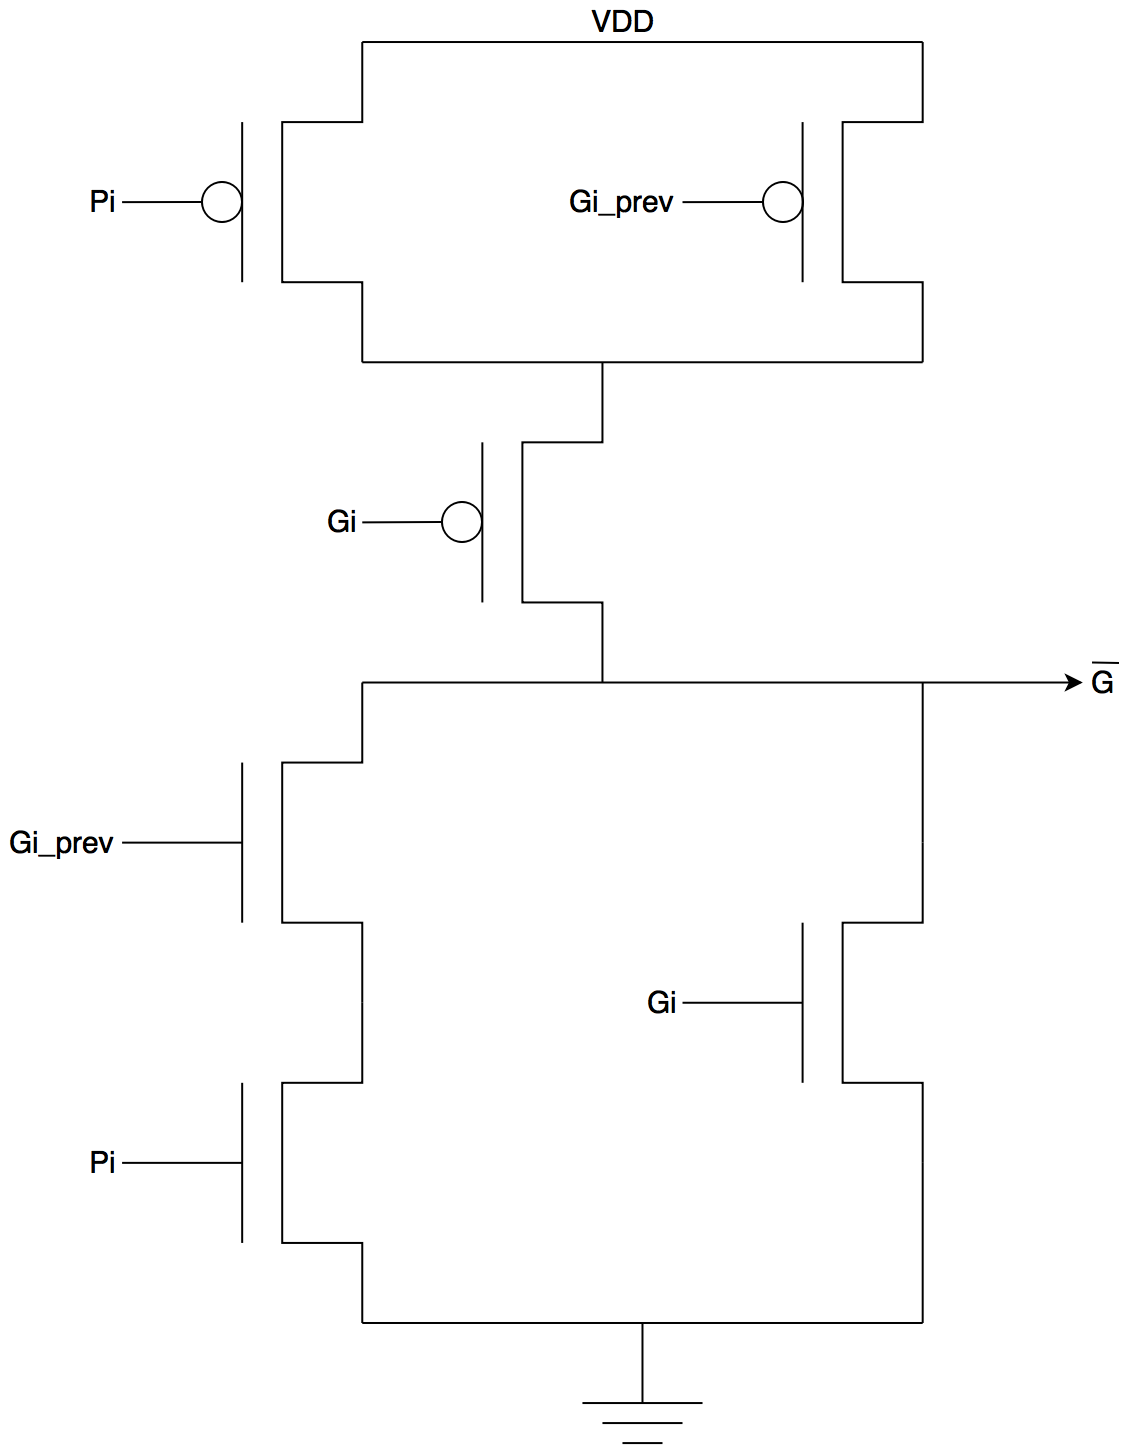
\includegraphics[scale=0.15]{../figures/G_inv_out}
  \caption{Generate part of \textit{yellow\_inv\_out}.} \label{fig:G_inv_out}
\end{figure}

